% !TXS template
\documentclass[12pt]{memoir}
\usepackage[T1]{fontenc}
\usepackage[utf8]{inputenc}
\usepackage{lmodern}
\usepackage[a4paper]{geometry}
\usepackage{graphics}
\usepackage{graphicx}
\usepackage{listings}
\usepackage{float}
\usepackage{hyperref}
\usepackage{multicol}
\setcounter{tocdepth}{3}
\setcounter{secnumdepth}{3}
\usepackage[font={small,it}]{caption}
%%\usepackage[margin=1.4in]{geometry}
%%\usepackage{babel}

%\addto\captionsfrench{% Replace "english" with the language you use
%	\renewcommand{\contentsname}%
%	{}%
%}
\renewcommand{\printtoctitle}[1]{\Huge \textbf{Table of Content}}

\renewcommand\thefigure{\arabic{figure}}
\renewcommand\thetable{\arabic{table}}
\setcounter{figure}{0}
\renewcommand{\thesection}{\arabic{section}}
\begin{document}

\title{Apprenticeship thesis, 2nd years \\ \textbf{Master of Computer Science}, speciality \textbf{Ingénierie du
		Logiciel et des Connaissances} 
	
	\bigskip
	{\huge Realtime continous optimisation of healthcare transportation fleets using massively parallele memetic algorithm on GPGPU} \\	
	}
\author{Joseph Pallamidessi\\ University of Strasbourg} 
\date{\vspace{2.5in}
	
\protect\raggedright
{\normalsize Maître d'alternance:} \\
		\textbf{Pierre Collet}, Université de Strasbourg \\
		\textbf{Guillaume Philips}, Synovo SAS}

\maketitle
\newpage

\tableofcontents*
\newpage


\section{Acknowlegments}\label{Acknowledgements}

I would first like to thank professor Collet, for the guidance provided during those
two year of apprenticeship. It is because of him that today I stand before you,
having opened to me the wonderful world of universitary research. \\
Guillaume Philip, my apprenticeship tutor inside Synovo to having me let experiment, test
and gave full liberty to conduit my research on this problem during the one and a
half year that I spent inside his company. He was always listening, throughful and
focus even when the obstacle seemed inreachable. He was flexibility, availability
and focus are something that I wish to encounter again in my carrier, as it gave me
the strength to finish this big challenge. \\
Jeremy Wies for my current position of research assistant at Synovo.
Thibault Thomas for his always optimistic mood and the overall help, on to many things to enumerate here. It was always a pleasure to discuss with him and I formally apologize for having him be me rubber ducks while being stuck on problems. As a true believer of the concept serendipity, many aspect of the current work may have been indirectly influenced by ours discussion. \\  
Benjamin Chetioui for having be an efficient and resourceful coworker and his numerous inputs in all aspects of this project.


\bigskip
I would like to thanks the pedagogic team of the ILC Master and more specifically M. Narboux, M. Magaud, Mme. Mark-Zwecker for allowing me to have this unorthodox journey through theirs formation, even if it had add a lot of supplementary work on them. \\
I would like to thanks Synovo and the ICube laboratories for their support and
letting me work in this big collaboration between university researchers and the
corporate world.
Thanks to all my proofreaders and friends for taking the time to help me and theirs overall support during those last two year. \\
Finally, I wish to thanks the french university and scholastic system for making me able to pursue my eduction.  
\newpage

\section{Abstract}
We developed a distributed multi-objectives genetic algorithm for solving a special case of
large vehicle routing for healthcare service. The goal of this algorithm is to
replace the task of planification for the next day currently done by human operator and with
minor modification,due to the evolutionary nature of the used techniques, be able to
done realtime continuous optimization. The problem in itself is highly constrained
but the search space remais large enough to require heuristics. The help the
exploitation phase, a set of local searches, the most used in combinatory
optimization have been reimplemented to take into account the specificities and
multi-objective nature of the problem. \\
The optimization must be fast enough with large instance to compete with humans as
this field is  caracterised by high frequence of modification through the day . In
order to avoid the traditional computational pitfall of pareto-based selection, a
novel selection method (G-ASREA) on GPGPU has been succesfully implemented and tested with
speed-up ranging for 4 to 50 times faster than the NSGAII algorithm while providing
better population diversity and overall results.
\paragraph{Keywords}
Evolutionary algorithm, genetic algorithm, local search, GPGPU, NSGA, ASREA, multi-objective optimization, pareto selection, vehicle routing problem with time windows, Pickup-delivery, heterogeneous fleet.
\newpage
\section{Introduction}
Planification of large instance remains an open field of research. The particular
problem of vehicle routing of healthcare service is twofolds : due to its
various constraints it is difficult to extract to ontology needed for modelizing for
a linear solver and the sheer number of element to optimize make it out of reach for
the classical exact algorithm, thus the need of powerful heuristics and 
metaheuristic. The fields af vehicle routing problem (VRP) is composed of numerous variants, each time defining new constraints. The two most commons one are the Capacited Vehicle Routing Problem (CVRP) and the Vehicle routing problem with time windows (VRPTW).

\paragraph{CVRP} % (fold)
\label{par:CVRP}
In the CVRP variant, the vehicle capacity of "goods" is limited and sometime the
good must also be package in the correct of delivery, meaning it involve a knapsack
optimisation once the routing is defined. This problem represent the core of
logistics and is prevalent in physical goods transportation. This is also the case
of our problem as theirs is a limited number of seat in the vehicles and some
limitation concerning the ambulances for example, where theirs can be only one
patient at once, independantly of the size of the medical crew.
% paragraph CVRP (end)
%Definition of CVRP

\paragraph{VRPTW} % (fold)
\label{par:VRPTW}
In the case of delivery to consumer directly arise the question of the delivery
timing. The VRPTW is a highly constrained problem where the delivery must occurs
at specific time window. Depending of the criticality of the delivery, systems tend
to treat windows with more or less flexibility. In our case, the delay penalty on an
appointement is weighted its type. The problem definition will be given in much more
detail in the following section.
% paragraph VRPTW (end)
%Definition of VRPTW

\paragraph{Heterogenous fleet} % (fold)
\label{par:Heterogenous fleet}
Problem with heterogenous fleet add a new set of constraints. The cost of using
the vehicle, its capacity, its crew (the size as well as the diploma and
authorization required) can depend of the type of vehicle.
% paragraph Heterogenous fleet (end)
%Variant one : heterogeouns fleet

\paragraph{Multi-depot} % (fold)
\label{par:Multi-depot}
The classical definition of the VRP problem state that theirs are only one depot or
main station, from which all the vehicle start and must go back after the last
missions. In the multi-depot variant, the vehicle are assigned to a specific base,
where they start and end.\\
% paragraph Multi-depot (end)
%Variant two : Multi-depot

The more constrained the problem is the smaller the search space will be. This fact
is easy to demonstrate when graphically solving a linear integer problem with the
simplex method for example.

%Genetic algorithm 
Distributed 

\section{Context of research}
\label{sec:Context of research}
The main motivation of this research is the automate the whole logistic process of
transporting patient for a number of reason. Historically healthcare transportation
services could not use any automation due to the large number of physicals and legal
constraints, in particular in France where the state subside part of the cost
depending on various complex conditions. This has render impossible the usage of
more traditional and top of the shelf solution available for the goods
transportation industry. Synovo, through its main product Saphir, an ERP-like tool
to manage the whole transporation company, try to push the full automation of the
industry. \\
The last remaining parts still extensibly done by humans operators are planning the
next day and doing realtime routing and problem solving during the day, two type of
work that our novel algorithm tackles efficently. The main goals to achieves are the
following:
\paragraph{Economic} % (fold)
\label{par:Economic}
A good planification that aggresively try to reduce the number of resources used
(vehicles, drivers, crews) can lead to massive saving for the transporation company
as well as improving the working condition of the current employee and preserving
the actual material.
% paragraph Economic (end)
\paragraph{Speed} % (fold)
\label{par:Speed}
For a small company, the average workload is about 100 to 200 missions (or journeys)
per day. For planning such day, it take around one hour very focused for a human
operator or regulator, while he is still interrupted by calls concerning the current
day. Before having a working planification for the next day, the company can not yet
tell its drivers and employees the beginning of theirs shifts. Having fast answer,
in the range of 5 minutes or less will be beneficial for the whole company.
% paragraph Speed (end)
\paragraph{Efficicy} % (fold)
\label{par:Efficicy}
Due to the high cognive demand of such work, the efficiency of the planning depend
in great part from the wellness of the regulator. While they are able to maintains
high quality planification during the work, the type of jobs is very exhausting on
the person. Algorithmic solutions will always have be constant in quality, and will
free the regulator to do its actual job of taking care of humans problem and
unforseeable incident on the field.

% paragraph Efficicy (end)

\subsection{Problem definition}
Formal definition

Difficulty of such optimisation : - Vehicle
- employee
Quality of result
-> two objective : load/legal + vehicle/employee
Patient => quality of service

\subsubsection{Healthcare transportation specificities}
\label{sub:Healthcare transportation specificities}
Priority on the quality of services and feasability
Pauses for employee
heterogeous fleet
Pick-up delivery


\section{State of the project}
Problem already finally defined 
Work already done
Small change => mainly refactoring
Genetic algorithm working fine 
In production

\section{Local searches}
Help the genetic algorithm with a set of local search
Exploitation/exploration
\subsection{2-opt* for pickup-delivery}
The exchange heuristic swaps two visits in differ-
ent routes. This is pictured in Figure 6. Finally, cross
is similar to 2-opt {\*}
proposed by Potvin and Rousseau
(1995) for VRPTW. Initially, a virtual vehicle, which
performs the visits not carried out by the real vehi-
cles, exists. This virtual vehicle is different from the
real  ones  in  two  respects.  First,  the  virtual  vehicle
can  make  an  unlimited  number  of  customer  visits.
Second, the cost incurred by the virtual vehicle when
it performs a customer visit is typically higher than
that incurred by a real vehicle.
\subsubsection{Base algorithm}
Enhancement of 2-opt
\subsubsection{PD-flavored version}

\subsection{Intra route}
Intra Route This heuristic picks two routes randomly and swaps two nodes from each route.
The nodes are chosen based on the numbers generated randomly. After the
swapping is done, feasibility is checked for the newly generated routes. If the
two new routes are acceptable, they will be updated as part of the solution;
otherwise the original routes will be restored.
\subsection{RAR}
Gendreau et al. [42] proposed a RAR (remove and
reinsert) mutation operator, which extracts a node and inserts it into a random point of
the routing sequence in order to retain the feasibility of solutions.
\subsection{Spliting and merging}
Route splitting and merging, nothing fancy here 
\subsection{Fuzzing}

\section{Result}
\subsection{Metrics definitions}
Focus on logistic and feasability : => no hard constraint violated
\subsection{G-ASREA vs NSGAII}
\subsubsection{Sélection et ranking : NSGAII et
	ASREA}\label{suxe9lection-et-ranking-nsgaii-et-asrea}

Une des grosses avancées de ces dernières semaines est le remplacement
de l'algorithme de sélection \emph{NSGA-II\cite{deb2002fast}} au profit d\emph{'ASREA\cite{sharma2010archived,tsutsui2013massively}}.\\
\emph{NSGA-II} est de facto l'algorithme de \emph{ranking} et de
sélection des \emph{MOEA}, avec une complexité asymptotique en O
(\emph{mn\^{}2}) avec \emph{m} nombre d'objectif et \emph{n} nombre
d'individu. Les implémentations en \emph{C/C++} de \emph{NSGA-II} sont
nombreuses, ce qui a justifié son choix dans un premier temps par M.
Catania.\\
Avec de grandes tailles de populations (\textgreater{}10 000
individus), le temps pris par \textit{NSGA-II} devient significatif par
rapport au reste de l'algorithme. Il se base sur le classement de rang
selon le principe de \textit{Pareto dominance} déjà évoqué plus haut. J'ai donc
décidé d'utiliser \textit{ASREA}, un algorithme de \textit{ranking} par archive
récent et innovant en O (\emph{man}) avec \emph{a} taille de l'archive ,
et sa variante parallélisée sur \emph{GPU}, \emph{G-ASREA\cite{sharma2010gpgpu}}.

\bigskip
\emph{NSGA,} comme \emph{ASREA}, propose une gestion de l'élitisme, le
premier par son classement déterministe de rang et le second par
l'utilisation d'une archive des meilleurs individus. Une explication
plus poussée des deux algorithmes est disponible en annexe. \\
Les accélérations d'\emph{ASREA} et \emph{G-ASREA} sont très
impressionnantes par rapport à \emph{NSGA-II}.
\begin{figure}[htbp]
	\begin{center}
		%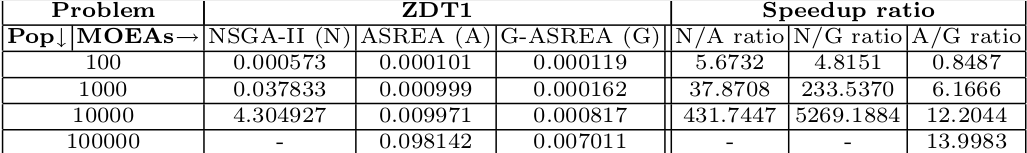
\includegraphics[width=6in]{img/asrea_table.png}
		\caption{Comparaison des temps et accélérations entre ASREA, NSGA-II et G-ASREA sur une minimisation de fonction ZDT\cite{zitzler2000comparison}.}
	\end{center}
\end{figure}
M. Collet m'a fourni une implémentation pour \textit{GPU} d'\emph{ASREA}. Le
code de l'algorithme était fortement imbriqué dans un programme de
benchmarking synthétique de \emph{GA} (\emph{ZDT functions\cite{zitzler2000comparison}}).

Nous avons continuer le travail de parallélisation sur \textit{G-ASREA} pour
qu'il soit exécuter en sont intégralité sur \textit{GPU}. Après extraction,
refactoring et adaptation, nous avons pu bénéficier d'accélérations
répertoriées dans la table suivante :

\begin{center}
	\begin{tabular}{ |l| c| r| }
		\hline
		Nombre d'individu & NSGA-II & G-ASREA \\
		\hline
		1024 & 5 ms & 2 ms \\
		16 384 & 464 ms & 19 ms\\
		32 768  & 1563 ms& 27 ms\\
		\hline
	\end{tabular}
	\captionof{table}{Temps de la sélection, moyennes sur 50 générations.}
\end{center}

\subsubsection{Execution time}
\subsubsection{Quality of results}

\paragraph{Per generations}

\paragraph{Observation}

\subsection{Comparaison against human operators}
Difficulty to do 

\section{Deployement}
CPU ok 
GPU => difficult 
Docker + AWS 

\section{Role}

\section{Discussion}

\section{Conclusion}

\nocite{*}
\bibliographystyle{plain}
\bibliography{mémoire}

\end{document}
